\documentclass[dvipsnames]{scrartcl}

\usepackage[margin=2.5cm]{geometry}

\makeatletter
\DeclareOldFontCommand{\rm}{\normalfont\rmfamily}{\mathrm}
\DeclareOldFontCommand{\sf}{\normalfont\sffamily}{\mathsf}
\DeclareOldFontCommand{\tt}{\normalfont\ttfamily}{\mathtt}
\DeclareOldFontCommand{\bf}{\normalfont\bfseries}{\mathbf}
\DeclareOldFontCommand{\it}{\normalfont\itshape}{\mathit}
\DeclareOldFontCommand{\sl}{\normalfont\slshape}{\@nomath\sl}
\DeclareOldFontCommand{\sc}{\normalfont\scshape}{\@nomath\sc}
\makeatother

\usepackage[dvipsnames]{xcolor}
\usepackage{tikz}

\usepackage{cmap} % allows copying math symbols from generated PDF
%\usepackage[only,grbassign]{stmaryrd}

\sloppy

\usepackage{hyperref} 
\usepackage{graphicx}

\usepackage{etoolbox}
\newbool{colored}
\boolfalse{colored}
\newbool{ascii}
\IfFileExists{./ascii}{\booltrue{ascii}}{\boolfalse{ascii}}

\usepackage{subcaption}
\usepackage{xspace}
\usepackage{booktabs}
\usepackage{enumitem}
\usepackage{numprint}
\usepackage{multirow}
\usepackage{xcolor}
\usepackage{todonotes}
\setuptodonotes{inline}

\hyphenation{Suite-Sparse}
\hyphenation{Graph-BLAS}
\hyphenation{Suite-Sparse-Graph-BLAS}

\newcommand{\suitesparse}{SuiteSparse\xspace}
\newcommand{\grb}{GraphBLAS\xspace}
\newcommand{\ssgrb}{SuiteSparse:GraphBLAS\xspace}
\newcommand{\gxb}{\ssgrb}
\newcommand{\lagraph}{LAGraph\xspace}
\newcommand{\pygrb}{pygraphblas\xspace}
\newcommand{\grblas}{grblas\xspace}

% Define new boolean flags using etoolbox ('\newbool' is similar to '\newtoggle').
% This workaround is needed as simply putting the newcommands inside 'IfFileExists' did not do the job
% as it broke with 'Illegal parameter number in definition of \reserved@a', a symptom probably caused
% by the lack of protection (\protect). Anyways, the workaround is actually cleaner.

%\newcommand{\grbreduce}[2]{\left[{#1}_j \, {#2}(:, j) \right]}
\ifbool{ascii}{
    \newcommand{\grbm}[1]{{\ifbool{colored}{\color{brown}}{}{\mathtt{#1}}}}% matrix
    \newcommand{\grbv}[1]{{\ifbool{colored}{\color{lilac}}{}{\mathtt{#1}}}}% vector
    \newcommand{\grba}[1]{{\ifbool{colored}{\color{gray}}{}{\mathtt{#1}}}}% array
    \newcommand{\grbs}[1]{{\ifbool{colored}{\color{blue}}{}{\mathtt{#1}}}}% scalar

    \newcommand{\grbstr}[1]{{\{#1\}}}
    \newcommand{\grbmask}[1]{<\! #1 \!>}
    \newcommand{\grbmaskreplace}[1]{<\!<\! #1 \!>\!>}
    \newcommand{\grbneg}{\texttt{!}}
    \newcommand{\grbassign}{\mathrel{\texttt{<-}}}
    \newcommand{\grbf}[2]{\grboperation{#1}(#2)}
    \newcommand{\grbreduce}[4]{[ {#1 #3} ]} % omit the indices
    \newcommand{\grbt}{\texttt{'}} % transpose
    \newcommand{\grbdiv}{\grbbinaryop{DIV}}
    \newcommand{\grbminus}{\grbbinaryop{MINUS}}
    \newcommand{\grbaccum}{\texttt{\ensuremath{+}}}
    \newcommand{\grbaccumeq}[1]{\mathbin{\texttt{\ensuremath{\ifstrempty{#1}{\grbaccum}{#1}=}}}}

    \newcommand{\grbplus}{\grbbinaryop{+}}
    \newcommand{\grbtimes}{\grbbinaryop{\times}}
    \newcommand{\grbapply}{\grbbinaryop{\odot}}

    \newcommand{\grbfrac}[2]{(#1)/(#2)}

    \newcommand{\grbbool}{\mathtt{bool}} % booleans
    \newcommand{\grbuint}{\mathtt{uint}} % unsigned integers
    \newcommand{\grbint}{\mathtt{int}}   % integers
    \newcommand{\grbfloat}{\mathtt{fp}}  % floats (?)

    \newcommand{\grbplaceholder}[1]{\mathsf{#1}}

    \newcommand{\grbscalartype}[2]{\mathtt{#1#2()}}
    \newcommand{\grbvectortype}[3]{\mathtt{#1#2(#3)}}
    \newcommand{\grbmatrixtype}[4]{\mathtt{#1#2(#3, #4)}}

    \newcommand{\grbnewscalar}[3]{\mathtt{#1 = \grbscalartype{#2}{#3}}}
    \newcommand{\grbnewvector}[4]{\mathtt{#1 = \grbvectortype{#2}{#3}{#4}}}
    \newcommand{\grbnewmatrix}[5]{\mathtt{#1 = \grbmatrixtype{#2}{#3}{#4}{#5}}}

    \newcommand{\grbalpha}{\mathtt{alpha}}
    \newcommand{\grboperator}[1]{\mathtt{#1}}

    \newcommand{\grbrange}[2]{#1:#2}
    \newcommand{\grbdontcare}{\_}

    \newcommand{\grboperationnoarg}[1]{\mathtt{#1}}
}{ % LaTeX mode
    \newcommand{\grbm}[1]{{\ifbool{colored}{\color{brown}}{}{\mathbf{#1}}}}% matrix
    \newcommand{\grbv}[1]{{\ifbool{colored}{\color{lilac}}{}{\mathbf{#1}}}}% vector
    %\newcommand{\grba}[1]{{\ifbool{colored}{\color{gray}}{}{\boldsymbol{#1}}}}% array
    \newcommand{\grba}[1]{{\ifbool{colored}{\color{gray}}{}{\textbf{\textit{#1}}}}}% array
    \newcommand{\grbs}[1]{{\ifbool{colored}{\color{blue}}{}{\mathit{#1}}}}% scalar

    \newcommand{\grbmask}[1]{\langle #1 \rangle}
    %\newcommand{\grbstr}[1]{{\{#1\}}}
    \newcommand{\grbstr}[1]{s(#1)}
    %\newcommand{\grbmaskreplace}[1]{\langle\!\langle #1 \rangle\!\rangle}
    \newcommand{\grbmaskreplace}[1]{\langle #1, \mathrm{r} \rangle}
    \newcommand{\grbneg}{\neg}

    % use the \mapsfrom symbol extracted from the stix package as suggested in https://tex.stackexchange.com/a/331899/71109
    \DeclareFontEncoding{LS1}{}{}
    \DeclareFontSubstitution{LS1}{stix}{m}{n}
    \DeclareSymbolFont{arrows1}{LS1}{stixsf}{m}{n}
    \global\let\mapsfrom\undefined % undefine \mapsfrom because some templates such as acmart already have it
    \DeclareMathSymbol{\mapsfrom}{\mathrel}{arrows1}{"AB}
    \newcommand{\grbassign}{\mapsfrom}

    \newcommand{\grbf}[2]{\grboperation{#1}{#2}}
    \newcommand{\grbreduce}[4]{[ {#1}_{#2}\, #3(#4) ]}
    \newcommand{\grbt}{^\mathsf{T}} %^{\top}} % transpose
    \newcommand{\grbdiv}{\grbbinaryop{\oslash}}
    \newcommand{\grbminus}{\grbbinaryop{\ominus}}
    \newcommand{\grbaccum}{\texttt{\ensuremath{\odot}}}
    \newcommand{\grbaccumeq}[1]{\mathbin{\ensuremath{\ifstrempty{#1}{\grbaccum}{#1}\!\!=}}}

    \newcommand{\grbplus}{\oplus}
    \newcommand{\grbtimes}{\otimes}
    \newcommand{\grbapply}{\odot}
    
    \newcommand{\grbfrac}[2]{\frac{#1}{#2}}

    \newcommand{\grbbool}{\mathbb{B}}  % booleans
    \newcommand{\grbuint}{\mathbb{N}}  % unsigned integers
    \newcommand{\grbint}{\mathbb{Z}}   % integers
    \newcommand{\grbfloat}{\mathbb{Q}} % floats (?)
    
    \newcommand{\grbplaceholder}[1]{\mathsf{#1}}

    \newcommand{\grbscalartype}[2]{#1_{#2}}
    \newcommand{\grbvectortype}[3]{#1_{#2}^{#3}}
    \newcommand{\grbmatrixtype}[4]{#1_{#2}^{#3 \times #4}}

    \newcommand{\grbnewscalar}[3]{\text{let: } #1 \in \grbscalartype{#2}{#3}}
    \newcommand{\grbnewvector}[4]{\text{let: } #1 \in \grbvectortype{#2}{#3}{#4}}
    \newcommand{\grbnewmatrix}[5]{\text{let: } #1 \in \grbmatrixtype{#2}{#3}{#4}{#5}}

    \newcommand{\grbalpha}{\alpha}
    \newcommand{\grboperator}[1]{\mathsf{#1}}

    \newcommand{\grbrange}[2]{#1 \! : \! #2}
    \newcommand{\grbdontcare}{\textvisiblespace}

    \newcommand{\grboperationnoarg}[1]{\textrm{#1}}
}

% do not lange/rangle for tuples as it is already used for masks
% do not use grbtuple for the time being
%\newcommand{\grbtuple}[1]{( #1 )}
\newcommand{\tuple}[1]{(#1)}

% trying to avoid too much syntax (e.g. using wedge/vee symbols for LAND/LOR)
%\newcommand{\grblorland}{\lor\!.\!\land}

\newcommand{\grbsemiringops}[2]{\mathbin{\grboperator{#1.#2}}}
\newcommand{\grbplustimes}{\grbsemiringops{\grbplus}{\grbtimes}}

\newcommand{\grbanypair}{\grbsemiringops{any}{pair}}
\newcommand{\grbanyfirst}{\grbsemiringops{any}{first}}
\newcommand{\grbanysecond}{\grbsemiringops{any}{second}}
\newcommand{\grbanyfirstj}{\grbsemiringops{any}{firstj}}
\newcommand{\grbanyfirstjone}{\grbsemiringops{any}{firstj1}}
\newcommand{\grbminfirstj}{\grbsemiringops{min}{firstj}}
\newcommand{\grbminfirstjone}{\grbsemiringops{min}{firstj1}}
\newcommand{\grbanysecondi}{\grbsemiringops{any}{secondi}}
\newcommand{\grbanysecondione}{\grbsemiringops{any}{secondi1}}
\newcommand{\grbminsecondi}{\grbsemiringops{min}{secondi}}
\newcommand{\grbminsecondione}{\grbsemiringops{min}{secondi1}}
\newcommand{\grblorland}{\grbsemiringops{lor}{land}}
\newcommand{\grbminplus}{\grbsemiringops{min}{plus}}
\newcommand{\grbmaxplus}{\grbsemiringops{max}{plus}}
\newcommand{\grbmaxfirst}{\grbsemiringops{max}{first}}
\newcommand{\grbminfirst}{\grbsemiringops{min}{first}}
\newcommand{\grbminsecond}{\grbsemiringops{min}{second}}
\newcommand{\grbmaxsecond}{\grbsemiringops{max}{second}}
\newcommand{\grbsecondmin}{\grbsemiringops{second}{min}}
\newcommand{\grbsecondmax}{\grbsemiringops{second}{max}}
\newcommand{\grbarithmeticplustimes}{\grbsemiringops{plus}{times}} % not necessary because this is the default

\newcommand{\grbbinaryop}[1]{\mathop{\grboperator{#1}}}
\newcommand{\grbany}{\grbbinaryop{any}}
\newcommand{\grbpair}{\grbbinaryop{pair}}
\newcommand{\grbland}{\grbbinaryop{land}}
\newcommand{\grblor}{\grbbinaryop{lor}}
\newcommand{\grbband}{\grbbinaryop{band}}
\newcommand{\grbbor}{\grbbinaryop{bor}}
\newcommand{\grbmin}{\grbbinaryop{min}}
\newcommand{\grbmax}{\grbbinaryop{max}}
\newcommand{\grbfirst}{\grbbinaryop{first}}
\newcommand{\grbsecond}{\grbbinaryop{second}}
\newcommand{\grbfirsti}{\grbbinaryop{firsti}}
\newcommand{\grbsecondi}{\grbbinaryop{secondi}}
\newcommand{\grbfirstione}{\grbbinaryop{firsti1}}
\newcommand{\grbsecondione}{\grbbinaryop{secondi1}}
\newcommand{\grbfirstj}{\grbbinaryop{firstj}}
\newcommand{\grbsecondj}{\grbbinaryop{secondj}}
\newcommand{\grbfirstjone}{\grbbinaryop{firstj1}}
\newcommand{\grbsecondjone}{\grbbinaryop{secondj1}}
\newcommand{\grbarithmeticplus}{\grbbinaryop{plus}} % usually not necessary because this is the default addition
\newcommand{\grbarithmetictimes}{\grbbinaryop{times}} % usually not necessary because this is the default multiplication
\newcommand{\grbisne}{\grbbinaryop{isne}}
\newcommand{\grbplustext}{\grbbinaryop{plus}}
\newcommand{\grbtimestext}{\grbbinaryop{times}}

% boolean values
\newcommand{\grbbooleanvalue}[1]{\mathtt{#1}}
\newcommand{\grbtrue}{\grbbooleanvalue{TRUE}}
\newcommand{\grbfalse}{\grbbooleanvalue{FALSE}}
\newcommand{\grbT}{\grbbooleanvalue{T}}
\newcommand{\grbF}{\grbbooleanvalue{F}}
\newcommand{\grbstring}{\textrm{String}}
\newcommand{\grbdate}{\textrm{Date}}

% cardinality / count
\newcommand{\grbcnt}[1]{| #1 |}

\newcommand{\grbeWiseAdd}[1]{\underset{\raisebox{.4ex}{$\scriptscriptstyle\cup$}}{#1}}
\newcommand{\grbeWiseMult}[1]{\underset{\raisebox{.4ex}{$\scriptscriptstyle\cap$}}{#1}}

% operations
\newcommand{\grboperation}[2]{\grboperationnoarg{#1}(#2)}
\newcommand{\grbnrows}[1]{\grboperation{nrows}{#1}}
\newcommand{\grbncols}[1]{\grboperation{ncols}{#1}}
\newcommand{\grbnvals}[1]{\grboperation{nvals}{#1}}
\newcommand{\grbclear}[1]{\grboperation{clear}{#1}}
\newcommand{\grbdiag}[1]{\grboperation{diag}{#1}}
\newcommand{\grbselect}[1]{\grbmask{#1}}
\newcommand{\grbkron}[1]{\grboperation{kron}{#1}}
\newcommand{\grbtril}[1]{\grboperation{tril}{#1}}
\newcommand{\grbtriu}[1]{\grboperation{triu}{#1}}
\newcommand{\grbondiag}[1]{\grboperation{ondiag}{#1}}
\newcommand{\grboffdiag}[1]{\grboperation{offdiag}{#1}}

\newcommand{\grbind}[1]{\mathrm{ind}(#1)}

\usetikzlibrary{matrix,arrows,decorations.pathmorphing}
\begin{document}


\begin{figure}
  \centering
  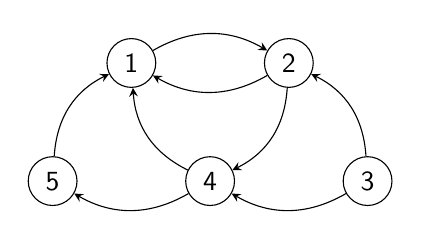
\begin{tikzpicture}[-stealth,align=center,every node/.style={circle, draw}]
      \sf % use sans-serif font
      \node[] at (1, 1.5) (V1) {1};
      \node[] at (3, 1.5) (V2) {2};
      \node[] at (4, 0) (V3) {3};
      \node[] at (2, 0) (V4) {4};
      \node[] at (0, 0) (V5) {5};
      \draw (V1) to [bend left] (V2);
      \draw (V2) to [bend left] (V1);
      \draw (V2) to [bend left] (V4);
      \draw (V3) to [bend right] (V2);
      \draw (V3) to [bend left] (V4);
      \draw (V4) to [bend left] (V1);
      \draw (V4) to [bend left] (V5);
      \draw (V5) to [bend left] (V1);


  \end{tikzpicture}
  \caption{Example directed graph.}
\end{figure}

%%%%%%%%%%%%%%%%%%%%%%%%%%%%%%%%%%%%%%%%%%%%%%%%%%%%%%%%%%%%%%%%%%%%%%%%%%%%%%%%
%%%%%%%%%%%%%%%%%%%%%%%%%%%%%%%%%%%%%%%%%%%%%%%%%%%%%%%%%%%%%%%%%%%%%%%%%%%%%%%%
%%%%%%%%%%%%%%%%%%%%%%%%%%%%%%%%%%%%%%%%%%%%%%%%%%%%%%%%%%%%%%%%%%%%%%%%%%%%%%%%

\newcommand{\myunit}{0.95cm}

\tikzset{
    node style sp/.style={draw,circle,minimum size=\myunit},
    node style ge/.style={circle,minimum size=\myunit},
%    arrow style addition/.style={midway,sloped,fill=white},
%    arrow style multiplication/.style={draw,sloped,midway,fill=white},
    arrow style addition/.style={midway,fill=white,inner sep=1pt},
    arrow style multiplication/.style={draw,midway,fill=white},
}

\begin{figure}
\centering
\begin{tikzpicture}[>=latex]
% 
\matrix (f) [matrix of math nodes,%
              nodes = {node style ge},%
              left delimiter  = {[},%
              right delimiter = {]}] at (0,3)
{%
|[node style sp,RoyalBlue]| 0 &
|[node style sp,RoyalBlue]| 1 &
|[node style sp,RoyalBlue]| 0 &
|[node style sp,RoyalBlue]| 1 &
|[node style sp,RoyalBlue]| 0 \\
};
\matrix (Ai) [matrix of math nodes,%
              nodes = {node style ge}] at (0,2)
{%
  \sf 1 & \sf 2 & \sf 3 & \sf 4 & \sf 5\\
};

\matrix (A) [matrix of math nodes,%
              nodes = {node style ge},%
              left delimiter  ={[},%
              right delimiter ={]}] at (6*\myunit,7*\myunit)
{%
  |[node style sp,RoyalBlue]| 0 & 1 & 0 & 0 & 0 \\
  |[node style sp,RoyalBlue]| 1 & 0 & 0 & 1 & 0 \\
  |[node style sp,RoyalBlue]| 0 & 1 & 0 & 1 & 0 \\
  |[node style sp,RoyalBlue]| 1 & 0 & 0 & 0 & 1 \\
  |[node style sp,RoyalBlue]| 1 & 0 & 0 & 0 & 0 \\
};
\matrix (Bi) [matrix of math nodes,%
              nodes = {node style ge}] at (9.5*\myunit,7*\myunit)
{%
  \sf 1 \\
  \sf 2 \\
  \sf 3 \\
  \sf 4 \\
  \sf 5 \\
};
\matrix (n) [matrix of math nodes,%
              nodes = {node style ge},%
              left delimiter  = {[},%
              right delimiter = {]}] at (6*\myunit,3)
{%
|[node style sp,RoyalBlue]| \tt 2 & \tt 0 & \tt 0 & \tt 1 & \tt 1 \\
};
\matrix (Ci) [matrix of math nodes,%
              nodes = {node style ge}] at (6*\myunit,2)
{%
  \sf 1 & \sf 2 & \sf 3 & \sf 4 & \sf 5\\
};

\tiny
\draw[-,RoyalBlue](f-1-1) to[in=180,out=90] node[arrow style multiplication] (x) {$0 \times 0 = 0$} (A-1-1);
\draw[-,RoyalBlue](f-1-2) to[in=180,out=90] node[arrow style multiplication] (y) {$1 \times 1 = 1$} (A-2-1);
\draw[-,RoyalBlue](f-1-3) to[in=180,out=90] node[arrow style multiplication] (z) {$0 \times 0 = 0$} (A-3-1);
\draw[-,RoyalBlue](f-1-4) to[in=180,out=90] node[arrow style multiplication] (w) {$1 \times 1 = 1$} (A-4-1);
\draw[-,RoyalBlue](f-1-5) to[in=180,out=90] node[arrow style multiplication] (v) {$0 \times 1 = 0$} (A-5-1);
\draw[RoyalBlue,->] (x)
  to node[arrow style addition] {\tiny $+$} (y)%
  to node[arrow style addition] {\tiny $+$} (z)%
  to node[arrow style addition] {\tiny $+$} (w)%
  to node[arrow style addition] {\tiny $+$} (v)%
  to (n-1-1.north west) ;

\end{tikzpicture}
\caption{Dense vector-matrix multiplication $\grbv{f} \grbm{A}$ on the conventional \textcolor{RoyalBlue}{$\grbsemiringops{+}{\times}$} semiring.}
\end{figure}

%%%%%%%%%%%%%%%%%%%%%%%%%%%%%%%%%%%%%%%%%%%%%%%%%%%%%%%%%%%%%%%%%%%%%%%%%%%%%%%%
%%%%%%%%%%%%%%%%%%%%%%%%%%%%%%%%%%%%%%%%%%%%%%%%%%%%%%%%%%%%%%%%%%%%%%%%%%%%%%%%
%%%%%%%%%%%%%%%%%%%%%%%%%%%%%%%%%%%%%%%%%%%%%%%%%%%%%%%%%%%%%%%%%%%%%%%%%%%%%%%%

\begin{figure}
\centering
\begin{tikzpicture}[>=latex]
% 
\matrix (f) [matrix of math nodes,%
              nodes = {node style ge},%
              left delimiter  = {[},%
              right delimiter = {]}] at (0,3)
{%
  \phantom{1} & |[node style sp,RoyalBlue]| 1 & \phantom{1} & |[node style sp,RoyalBlue]| 1 & \phantom{1} \\
};
\matrix (Ai) [matrix of math nodes,%
              nodes = {node style ge}] at (0,2)
{%
  \sf 1 & \sf 2 & \sf 3 & \sf 4 & \sf 5\\
};

\matrix (A) [matrix of math nodes,%
              nodes = {node style ge},%
              left delimiter  ={[},%
              right delimiter ={]}] at (6*\myunit,7*\myunit)
{%
                        &     1 & \vphantom{.} &       &       \\
|[node style sp,RoyalBlue]|     1 &       &        &     1 &       \\
                        &     1 &        &     1 &       \\
|[node style sp,RoyalBlue]|     1 &       &        &       &     1 \\
                      1 &       &        &       &       \\
};
\matrix (Bi) [matrix of math nodes,%
              nodes = {node style ge}] at (9.5*\myunit,7*\myunit)
{%
  \sf 1 \\
  \sf 2 \\
  \sf 3 \\
  \sf 4 \\
  \sf 5 \\
};
%
\matrix (n) [matrix of math nodes,%
              nodes = {node style ge},%
              left delimiter  = {[},%
              right delimiter = {]}] at (6*\myunit,3)
{%
|[node style sp,RoyalBlue]| \tt 2 & \ & \ & \tt 1 & \tt 1 \\
};
\matrix (Ci) [matrix of math nodes,%
              nodes = {node style ge}] at (6*\myunit,2)
{%
  \sf 1 & \sf 2 & \sf 3 & \sf 4 & \sf 5\\
};

\draw[-,RoyalBlue](f-1-2) to[in=180,out=90] node[arrow style multiplication] (x) {$1 \times 1 = \tt 1$} (A-2-1);
\draw[-,RoyalBlue](f-1-4) to[in=180,out=90] node[arrow style multiplication] (y) {$1 \times 1 = \tt 1$} (A-4-1);
\draw[RoyalBlue,->] (x)
  to node[arrow style addition] {$+$} (y)%
  to (n-1-1.north west) ;

\end{tikzpicture}
\caption{Sparse vector-matrix multiplication $\grbv{f} \grbm{A}$ on the conventional \textcolor{RoyalBlue}{$\grbsemiringops{+}{\times}$} semiring.}
\end{figure}

%%%%%%%%%%%%%%%%%%%%%%%%%%%%%%%%%%%%%%%%%%%%%%%%%%%%%%%%%%%%%%%%%%%%%%%%%%%%%%%%
%%%%%%%%%%%%%%%%%%%%%%%%%%%%%%%%%%%%%%%%%%%%%%%%%%%%%%%%%%%%%%%%%%%%%%%%%%%%%%%%
%%%%%%%%%%%%%%%%%%%%%%%%%%%%%%%%%%%%%%%%%%%%%%%%%%%%%%%%%%%%%%%%%%%%%%%%%%%%%%%%

\begin{figure}
\centering
\begin{tikzpicture}[>=latex]
% 
\matrix (f) [matrix of math nodes,%
              nodes = {node style ge},%
              left delimiter  = {[},%
              right delimiter = {]}] at (0,3)
{%
  \phantom{\grbT} & |[node style sp,OliveGreen]| \grbT & \phantom{\grbT} & |[node style sp,OliveGreen]| \grbT & \phantom{\grbT} \\
};
\matrix (Ai) [matrix of math nodes,%
              nodes = {node style ge}] at (0,2)
{%
  \sf 1 & \sf 2 & \sf 3 & \sf 4 & \sf 5\\
};

\matrix (A) [matrix of math nodes,%
              nodes = {node style ge},%
              left delimiter  ={[},%
              right delimiter ={]}] at (6*\myunit,7*\myunit)
{%
                        & \grbT & \vphantom{.} &       &       \\
|[node style sp,OliveGreen]| \grbT &       &        & \grbT &       \\
                        & \grbT &        & \grbT &       \\
|[node style sp,OliveGreen]| \grbT &       &        &       & \grbT \\
                  \grbT &       &        &       &       \\
};
\matrix (Bi) [matrix of math nodes,%
              nodes = {node style ge}] at (9.5*\myunit,7*\myunit)
{%
  \sf 1 \\
  \sf 2 \\
  \sf 3 \\
  \sf 4 \\
  \sf 5 \\
};
%
\matrix (n) [matrix of math nodes,%
              nodes = {node style ge},%
              left delimiter  = {[},%
              right delimiter = {]}] at (6*\myunit,3)
{%
|[node style sp,OliveGreen]| \tt \grbT & \ & \ & \tt \grbT & \tt \grbT \\
};
\matrix (Ci) [matrix of math nodes,%
              nodes = {node style ge}] at (6*\myunit,2)
{%
  \sf 1 & \sf 2 & \sf 3 & \sf 4 & \sf 5\\
};

\draw[-,OliveGreen](f-1-2) to[in=180,out=90] node[arrow style multiplication] (x) {$\grbT \, \grbland \, \grbT = \grbT$} (A-2-1);
\draw[-,OliveGreen](f-1-4) to[in=180,out=90] node[arrow style multiplication] (y) {$\grbT \, \grbland \, \grbT = \grbT$} (A-4-1);
\draw[OliveGreen,->] (x)
  to node[arrow style addition] {$\grblor$} (y)%
  to (n-1-1.north west) ;

\end{tikzpicture}
\caption{Sparse vector-matrix multiplication $\grbv{f} \grbm{A}$ on the \textcolor{OliveGreen}{$\grblorland$} ($\vee.\wedge$) semiring.}
\end{figure}

%%%%%%%%%%%%%%%%%%%%%%%%%%%%%%%%%%%%%%%%%%%%%%%%%%%%%%%%%%%%%%%%%%%%%%%%%%%%%%%%
%%%%%%%%%%%%%%%%%%%%%%%%%%%%%%%%%%%%%%%%%%%%%%%%%%%%%%%%%%%%%%%%%%%%%%%%%%%%%%%%
%%%%%%%%%%%%%%%%%%%%%%%%%%%%%%%%%%%%%%%%%%%%%%%%%%%%%%%%%%%%%%%%%%%%%%%%%%%%%%%%

\begin{figure}
\centering
\begin{tikzpicture}[>=latex]
% 
\matrix (f) [matrix of math nodes,%
              nodes = {node style ge},%
              left delimiter  = {[},%
              right delimiter = {]}] at (0,3)
{%
  \phantom{\grbT} & |[node style sp,RubineRed]| \grbT & \phantom{\grbT} & |[node style sp,RubineRed]| \grbT & \phantom{\grbT} \\
};
\matrix (Ai) [matrix of math nodes,%
              nodes = {node style ge}] at (0,2)
{%
  \sf 1 & \sf 2 & \sf 3 & \sf 4 & \sf 5\\
};

\matrix (A) [matrix of math nodes,%
              nodes = {node style ge},%
              left delimiter  ={[},%
              right delimiter ={]}] at (6*\myunit,7*\myunit)
{%
                            & \grbT        & \vphantom{.} &       &       \\
|[node style sp,RubineRed]| \grbT &              &              & \grbT &       \\
                            & \grbT        &              & \grbT &       \\
|[node style sp,RubineRed]| \grbT &              &              &       & \grbT \\
                      \grbT &              &              &       &       \\
};
\matrix (Bi) [matrix of math nodes,%
              nodes = {node style ge}] at (9.5*\myunit,7*\myunit)
{%
  \sf 1 \\
  \sf 2 \\
  \sf 3 \\
  \sf 4 \\
  \sf 5 \\
};
%
\matrix (n) [matrix of math nodes,%
              nodes = {node style ge},%
              left delimiter  = {[},%
              right delimiter = {]}] at (6*\myunit,3)
{%
|[node style sp,RubineRed]| \tt \grbT & \ & \ & \tt \grbT & \tt \grbT \\
};
\matrix (Ci) [matrix of math nodes,%
              nodes = {node style ge}] at (6*\myunit,2)
{%
  \sf 1 & \sf 2 & \sf 3 & \sf 4 & \sf 5\\
};

%\draw[-,RubineRed](f-1-2) to[in=180,out=90] node[arrow style multiplication] (x) {$\grbv{f}(2) \, \grbpair \, \grbm{A}(\sf 2, 1) = \grbT$} (A-2-1);
%\draw[-,RubineRed](f-1-4) to[in=180,out=90] node[arrow style multiplication] (y) {$\grbv{f}(4) \, \grbpair \, \grbm{A}(\sf 4, 1) = \grbT$} (A-4-1);
\draw[-,RubineRed](f-1-2) to[in=180,out=90] node[arrow style multiplication] (x) {$\grbdontcare \, \grbpair \, \grbdontcare = \grbT$} (A-2-1);
\draw[-,RubineRed](f-1-4) to[in=180,out=90] node[arrow style multiplication] (y) {$\grbdontcare \, \grbpair \, \grbdontcare = \grbT$} (A-4-1);
\draw[RubineRed,->] (x)
  to node[arrow style addition] {$\grbany$} (y)%
  to (n-1-1.north west) ;

\end{tikzpicture}
\caption{Sparse vector-matrix multiplication $\grbv{f} \grbm{A}$ on the \textcolor{RubineRed}{$\grbanypair$} semiring (currently only available in \gxb). The \emph{don't-care} values are denoted with the $\grbdontcare$ symbol.}
\end{figure}

%%%%%%%%%%%%%%%%%%%%%%%%%%%%%%%%%%%%%%%%%%%%%%%%%%%%%%%%%%%%%%%%%%%%%%%%%%%%%%%%
%%%%%%%%%%%%%%%%%%%%%%%%%%%%%%%%%%%%%%%%%%%%%%%%%%%%%%%%%%%%%%%%%%%%%%%%%%%%%%%%
%%%%%%%%%%%%%%%%%%%%%%%%%%%%%%%%%%%%%%%%%%%%%%%%%%%%%%%%%%%%%%%%%%%%%%%%%%%%%%%%

\begin{figure}
  \centering
  \begin{tikzpicture}[>=latex]
  % 
  \matrix (f) [matrix of math nodes,%
                nodes = {node style ge},%
                left delimiter  = {[},%
                right delimiter = {]}] at (0,3)
  {%
    \phantom{\grbT} & |[node style sp,Plum]| \grbT & \phantom{\grbT} & |[node style sp,Plum]| \grbT & \phantom{\grbT} \\
  };
  \matrix (Ai) [matrix of math nodes,%
                nodes = {node style ge}] at (0,2)
  {%
    \sf 1 & \sf 2 & \sf 3 & \sf 4 & \sf 5\\
  };
  
  \matrix (A) [matrix of math nodes,%
                nodes = {node style ge},%
                left delimiter  ={[},%
                right delimiter ={]}] at (6*\myunit,7*\myunit)
  {%
                            & \grbT & \vphantom{.} &       &       \\
    |[node style sp,Plum]| \grbT &       &        & \grbT &       \\
                            & \grbT &        & \grbT &       \\
    |[node style sp,Plum]| \grbT &       &        &       & \grbT \\
                      \grbT &       &        &       &       \\
  };
  \matrix (Bi) [matrix of math nodes,%
                nodes = {node style ge}] at (9.5*\myunit,7*\myunit)
  {%
    \sf 1 \\
    \sf 2 \\
    \sf 3 \\
    \sf 4 \\
    \sf 5 \\
  };
  
  \matrix (n) [matrix of math nodes,%
                nodes = {node style ge},%
                left delimiter  = {[},%
                right delimiter = {]}] at (6*\myunit,3)
  {%
  |[node style sp,Plum]| \tt 2 & \ & \ & \tt 2 & \tt 4 \\
  };
  \matrix (Ci) [matrix of math nodes,%
                nodes = {node style ge}] at (6*\myunit,2)
  {%
    \sf 1 & \sf 2 & \sf 3 & \sf 4 & \sf 5\\
  };
  
  % les fleches
  \draw[-,Plum](f-1-2) to[in=180,out=90] node[arrow style multiplication] (x) {$\grbv{f}(2) \, \grbsecondione \, \grbm{A}(\sf 2, 1) = \tt 2$} (A-2-1);
  \draw[-,Plum](f-1-4) to[in=180,out=90] node[arrow style multiplication] (y) {$\grbv{f}(4) \, \grbsecondione \, \grbm{A}(\sf 4, 1) = \tt 4$} (A-4-1);
  \draw[Plum,->] (x)
    to node[arrow style addition] {$\grbmin$} (y)%
    to (n-1-1.north west) ;
  
  \end{tikzpicture}
  \caption{Sparse vector-matrix multiplication $\grbv{f} \grbm{A}$ on the \textcolor{Plum}{$\grbminsecondione$} %{$\grbminfirstjone$}
  semiring (only available in \gxb).
  %The $\grbfirstjone$ operator returns the column index of the first operand using 1-based indexing.
  The $\grbsecondione$ operator returns the row index of the element in the second operand using 1-based indexing.
  }
\end{figure}

%%%%%%%%%%%%%%%%%%%%%%%%%%%%%%%%%%%%%%%%%%%%%%%%%%%%%%%%%%%%%%%%%%%%%%%%%%%%%%%%
%%%%%%%%%%%%%%%%%%%%%%%%%%%%%%%%%%%%%%%%%%%%%%%%%%%%%%%%%%%%%%%%%%%%%%%%%%%%%%%%
%%%%%%%%%%%%%%%%%%%%%%%%%%%%%%%%%%%%%%%%%%%%%%%%%%%%%%%%%%%%%%%%%%%%%%%%%%%%%%%%

\begin{figure}
  \centering
  \begin{tikzpicture}[>=latex]
  % 
  \matrix (f) [matrix of math nodes,%
                nodes = {node style ge},%
                left delimiter  = {[},%
                right delimiter = {]}] at (0,3)
  {%
    \phantom{\grbT} & |[node style sp,Plum]| \grbT & \phantom{\grbT} & |[node style sp,Plum]| \grbT & \phantom{\grbT} \\
  };
  \matrix (Ai) [matrix of math nodes,%
                nodes = {node style ge}] at (0,2)
  {%
    \sf 1 & \sf 2 & \sf 3 & \sf 4 & \sf 5\\
  };
  
  \matrix (A) [matrix of math nodes,%
                nodes = {node style ge},%
                left delimiter  ={[},%
                right delimiter ={]}] at (6*\myunit,7*\myunit)
  {%
                            & \grbT & \vphantom{.} &       &       \\
    |[node style sp,Plum]| \grbT &       &        & \grbT &       \\
                            & \grbT &        & \grbT &       \\
    |[node style sp,Plum]| \grbT &       &        &       & \grbT \\
                      \grbT &       &        &       &       \\
  };
  \matrix (Bi) [matrix of math nodes,%
                nodes = {node style ge}] at (9.5*\myunit,7*\myunit)
  {%
    \sf 1 \\
    \sf 2 \\
    \sf 3 \\
    \sf 4 \\
    \sf 5 \\
  };
  
  \matrix (n) [matrix of math nodes,%
                nodes = {node style ge},%
                left delimiter  = {[},%
                right delimiter = {]}] at (6*\myunit,3)
  {%
  |[node style sp,Plum]| \tt 2 & \ & \ & \tt 2 & \tt 4 \\
  };
  \matrix (Ci) [matrix of math nodes,%
                nodes = {node style ge}] at (6*\myunit,2)
  {%
    \sf 1 & \sf 2 & \sf 3 & \sf 4 & \sf 5\\
  };
  
    % \draw[-,Plum](f-1-2) to[in=180,out=90] node[arrow style multiplication] (x) {$\grbv{f}(2) \, \grbsecondione \, \grbm{A}(\sf 2, 1) = \tt 2$} (A-2-1);
  % \draw[-,Plum](f-1-4) to[in=180,out=90] node[arrow style multiplication] (y) {$\grbv{f}(4) \, \grbsecondione \, \grbm{A}(\sf 4, 1) = \tt 4$} (A-4-1);
  % \draw[-,Plum](f-1-2) to[in=180,out=90] node[arrow style multiplication] (x) {$\grbdontcare \, \grbsecondione \, \grbdontcare = \tt 2$} (A-2-1);
  % \draw[-,Plum](f-1-4) to[in=180,out=90] node[arrow style multiplication] (y) {$\grbdontcare \, \grbsecondione \, \grbdontcare = \tt 4$} (A-4-1);
  \draw[-,Plum](f-1-2) to[in=180,out=90] node[arrow style multiplication] (x) {$\grbsecondione(\grbdontcare, \grbdontcare) = \tt 2$} (A-2-1);
  \draw[-,Plum](f-1-4) to[in=180,out=90] node[arrow style multiplication] (y) {$\grbsecondione(\grbdontcare, \grbdontcare) = \tt 4$} (A-4-1);
  \draw[Plum,->] (x)
    to node[arrow style addition] {$\grbmin$} (y)%
    to (n-1-1.north west) ;
  
  \end{tikzpicture}
  \caption{Sparse vector-matrix multiplication $\grbv{f} \grbm{A}$ on the \textcolor{Plum}{$\grbminsecondione$} %{$\grbminfirstjone$}
  semiring (only available in \gxb).
  %The $\grbfirstjone$ operator returns the column index of the first operand using 1-based indexing.
  The $\grbsecondione$ operator returns the row index of the element in the second operand using 1-based indexing. This figure uses \emph{don't-care} values ($\grbdontcare$).
  }
\end{figure}


\end{document}
